% =====================================================================
% §3 DEFINIÇÃO E MODELAGEM DO PROBLEMA
% Formulação completa + chaves visuais (agenda, troca, gamma)
% =====================================================================
\section{Formalização e Modelagem do Problema}

%%% Frame 3.1 — Contextualização + hipóteses
\begin{frame}{Contextualização do problema}

    \begin{block}{O que é pedido}
        Construir a agenda de trabalho de \textbf{múltiplas unidades} para todos os médicos ao longo do horizonte, respeitando disponibilidade, demanda e capacidade de salas.
    \end{block}

    \begin{figure}
        \centering
        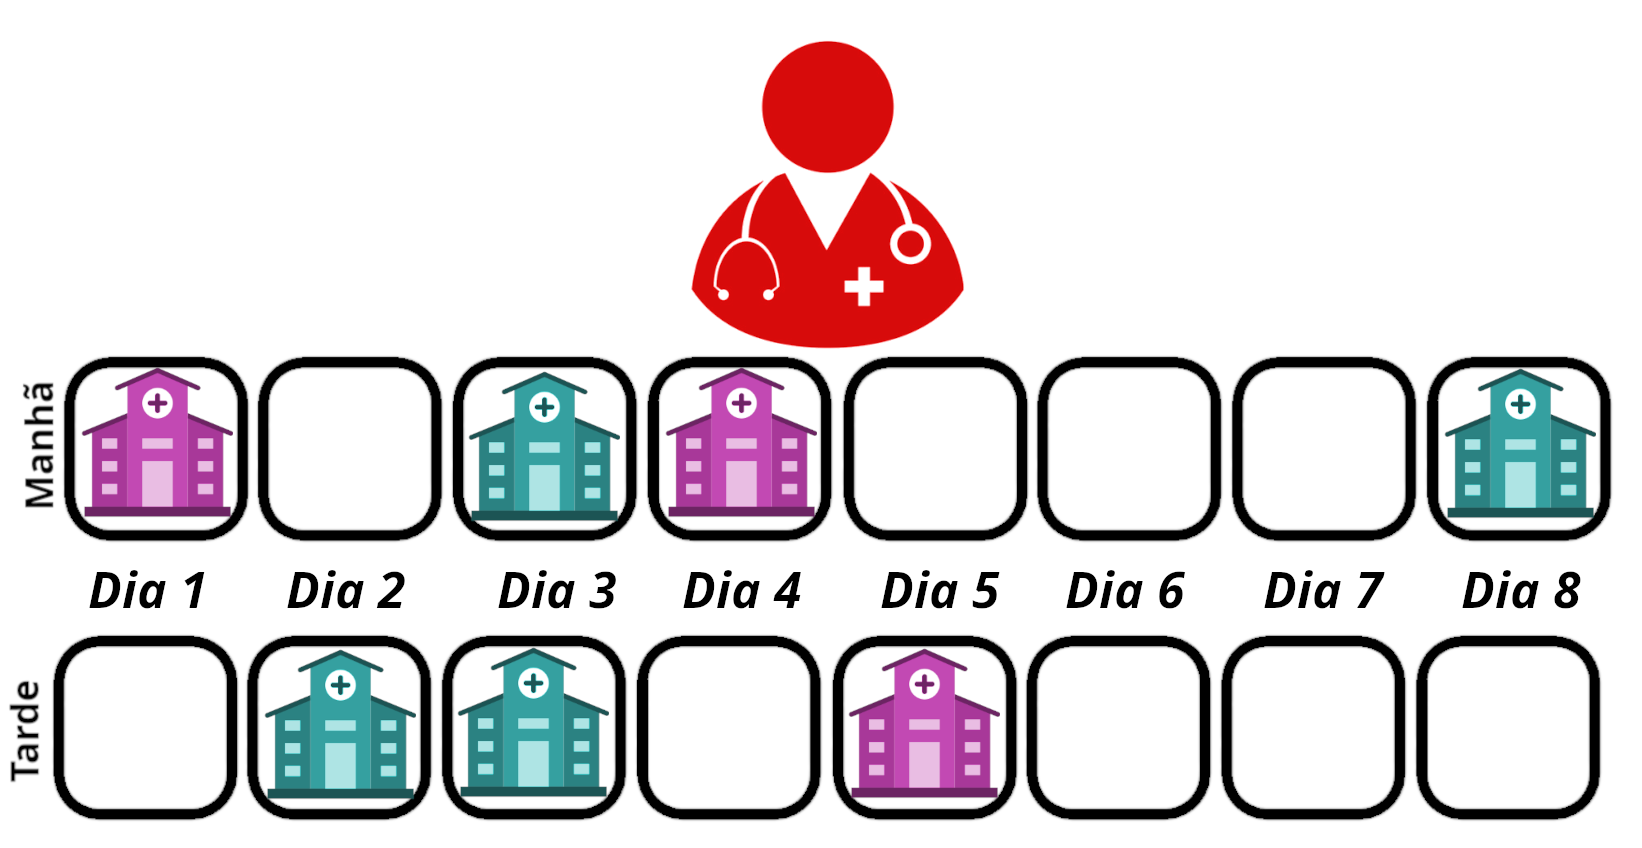
\includegraphics[width=0.46\linewidth]{img/exemplo-schedule-medico.png}
        \caption{Exemplo de agenda de um médico (chave visual).}
        \label{fig:ex-agenda}
    \end{figure}
    % TODO: 15 min/exame \cite{conselho_regional_de_medicina_do_estado_do_parana_2022};
    %       dados estáticos, obtidos em acordo com a rede.
\end{frame}

%%% Frame 3.2 — Hipóteses de modelagem
\begin{frame}{Hipóteses de modelagem}
    \begin{footnotesize}
        \begin{longtable}[l]{cl}
            \multicolumn{2}{l}{\textbf{Regras de negócio $\rightarrow$ hipóteses (H1--H7)}} \\[2pt]
            \textit{H1} & Todas as clínicas atendidas, mesmo com cobertura mínima. \\
            \textit{H2} & Um médico associado a apenas uma unidade por dia. \\
            \textit{H3} & Cada médico associado a uma sala da clínica. \\
            \textit{H4} & Médico realiza quantidade de exames conforme demanda da unidade. \\
            \textit{H5} & Diferença atendimentos $\times$ demanda = exames não atendidos. \\
            \textit{H6} & Agenda irregular: sem limite de remanejamentos entre clínicas. \\
            \textit{H7} & Dada condição inicial (histórico), minimizam-se remanejamentos. \\
        \end{longtable}
    \end{footnotesize}
    % TODO: H6/H7 motivam a FO2 e a variável de estado gamma.
\end{frame}

%%% Frame 3.3 — Índices, parâmetros e variáveis
\begin{frame}{Componentes do problema}
    \begin{small}
        \begin{longtable}[l]{lllll}
            \multicolumn{5}{l}{\textbf{Índices e conjuntos}} \\
            $i \in I$ & Médicos & \quad & $t \in T$ & Turnos \\
            $u \in U$ & Unidades & \quad & $I_u$ & Médicos que atendem em $u$ \\
            $d \in D$ & Dias & \quad & $U_i$ & Unidades atendidas por $i$ \\
        \end{longtable}

        \begin{longtable}[l]{ll}
            \multicolumn{2}{l}{\textbf{Parâmetros}} \\
            $e_{udt}$ & Demanda por exames em $u$, dia $d$, turno $t$ \\
            $s_{udt}$ & Salas disponíveis em $u$, dia $d$, turno $t$ \\
            $q_{idt}$ & Exames que o médico $i$ realiza em $d,t$ \\
            $a_{idt}$ & Disponibilidade do médico $i$ em $d,t$ \\
        \end{longtable}

        \begin{longtable}[l]{ll}
            \multicolumn{2}{l}{\textbf{Variáveis}} \\
            $x_{iudt}$ & $1$ se $i$ alocado em $u$, dia $d$, turno $t$ \\
            $w_{iud}$ & $1$ se $i$ alocado em $u$ no dia $d$ \\
            $c_{udt}$ & Exames não atendidos em $u,d,t$ \\
            $z_{id}$ & $1$ se $i$ trocou de clínica no dia $d$ \\
        \end{longtable}
    \end{small}
\end{frame}

%%% Frame 3.4 — Restrições estruturais R1-R6
\begin{frame}{Restrições estruturais}
    \resizebox{\textwidth}{!}{\begin{minipage}{1.25\textwidth}
        \begin{alignat}{2}
            \sum_{u \in U_i} x_{iudt} \leq a_{idt} \quad & \forall i \in I, d \in D, t \in T \label{eq:r1} \\
            \sum_{u \in U_i} w_{iud} \leq 1 \quad & \forall i \in I, d \in D \label{eq:r2} \\
            x_{iudt} \leq w_{iud} \quad & \forall i \in I, u \in U, d \in D, t \in T \label{eq:r3} \\
            w_{iud} = 0 \quad & \forall i \in I, u \notin U_i, d \in D \label{eq:r4} \\
            \sum_{i \in I_u} x_{iudt} \leq s_{udt} \quad & \forall u \in U, d \in D, t \in T \label{eq:r5} \\
            \sum_{i \in I_u} x_{iudt} \geq b_{udt} \quad & \forall u \in U, d \in D, t \in T \label{eq:r6} \\
            x_{iudt}, w_{iud} \in \{0,1\} \quad & \forall i,u,d,t \label{eq:dom}
        \end{alignat}
    \end{minipage}}

    % TODO chave visual: R1 disponibilidade | R2-R3 unicidade diária |
    %      R4 elegibilidade | R5 capacidade de salas | R6 cobertura mínima.
\end{frame}

%%% Frame 3.5 — FO1 exames não atendidos
\begin{frame}{$Z_1$ — Minimizar exames não atendidos}
    \resizebox{\textwidth}{!}{\begin{minipage}{1.2\textwidth}

        \begin{block}{Motivação}
            Cobertura da operação e fluxo de caixa da rede.
        \end{block}

        \begin{equation}
            \min \sum_{u \in U}\sum_{d \in D}\sum_{t \in T} c_{udt} \label{eq:fo1}
        \end{equation}
        \hspace{1.5cm} sujeito a:
        \begin{alignat}{2}
            c_{udt} \geq e_{udt} - \sum_{i \in I_u}(q_{idt} \cdot x_{iudt}) \quad & \forall u \in U, d \in D, t \in T \label{eq:fo1-r1} \\
            c_{udt} \in \mathbb{Z}^{*}_{+} \quad & \forall u \in U, d \in D, t \in T \label{eq:fo1-dom}
        \end{alignat}
    \end{minipage}}
\end{frame}

%%% Frame 3.6 — FO2 trocas + problema das lacunas
\begin{frame}{$Z_2$ — Minimizar trocas de clínica}
    \begin{block}{Motivação}
        Ergonomia e estabilidade da agenda do profissional.
    \end{block}
    \begin{figure}
        \centering
        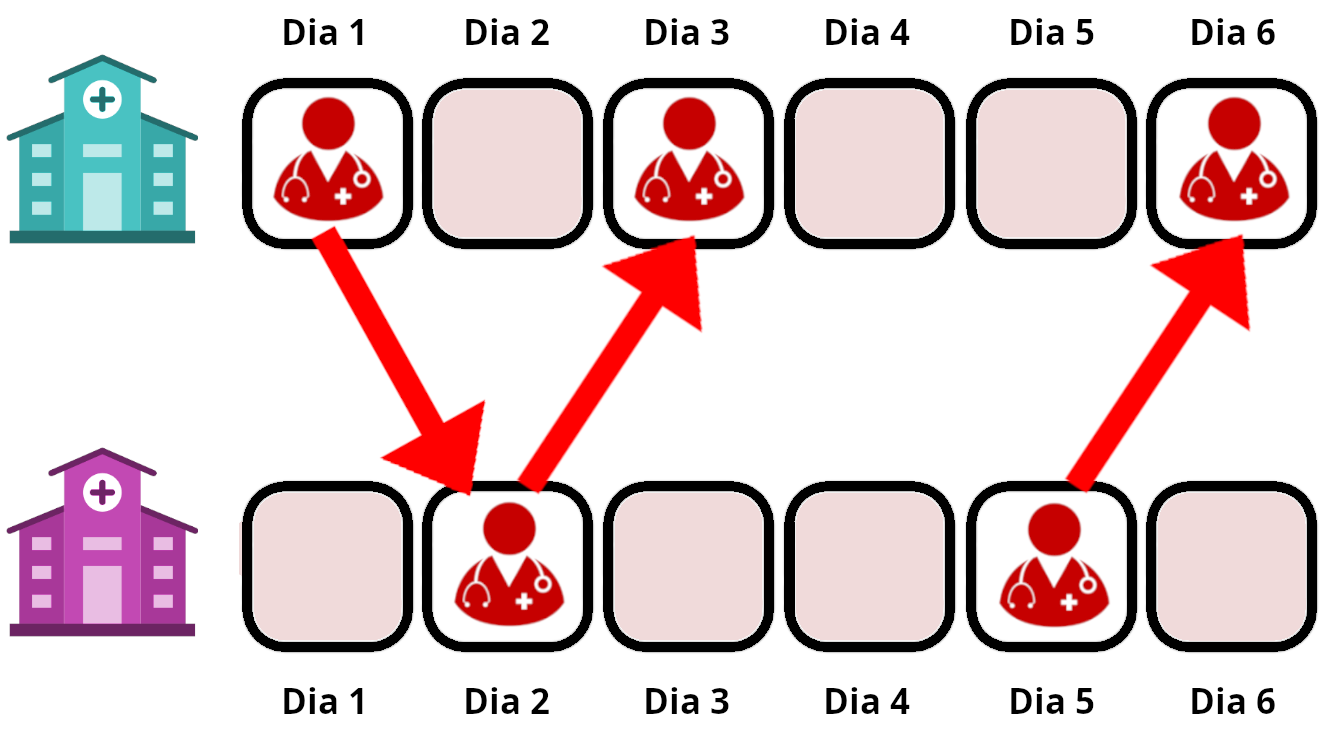
\includegraphics[width=0.55\linewidth]{img/troca-examplo.png}
        \caption{Exemplo de troca em uma agenda (chave visual).}
        \label{fig:ex-troca}
    \end{figure}
    \begin{block}{Desafio}
        Agendas irregulares têm \textbf{lacunas} (dias sem trabalho). Comparar dias consecutivos falha em detectar trocas através das lacunas.
    \end{block}
\end{frame}

%%% Frame 3.7 — variável de estado gamma (peça central)
\begin{frame}{Variável de estado $\gamma_{iud}$ — detecção de trocas}
    \begin{columns}[T]
        \begin{column}{0.5\textwidth}
            \begin{block}{Ideia (adaptada do GLSP \cite{Fleischmann_Meyr_1997})}
                $\gamma_{iud}$ registra a clínica em que o médico está \emph{conceitualmente}, mesmo sem alocação ativa; o estado \textbf{persiste} nas lacunas.
            \end{block}
            \resizebox{\linewidth}{!}{\begin{minipage}{1.15\linewidth}
                \begin{alignat}{2}
                    \gamma_{iud} \geq w_{iud} & \label{eq:g-def} \\
                    \sum_{u \in U_i} \gamma_{iud} = 1 & \label{eq:g-sum} \\
                    z_{id} \geq \gamma_{iud} + \!\!\sum_{u' \neq u}\! \gamma_{i,u',d-1} - 1 & \label{eq:g-swap}
                \end{alignat}
            \end{minipage}}
        \end{column}
        \begin{column}{0.5\textwidth}
            \begin{figure}
                \centering
                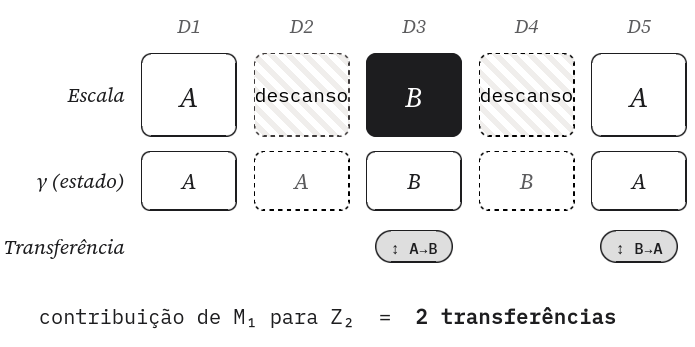
\includegraphics[width=\linewidth]{img/04_nsga-05_gama.png}
                \caption{Estado $\gamma_{iud}$ ao longo dos dias.}
                \label{fig:gamma}
            \end{figure}
        \end{column}
    \end{columns}
    \begin{footnotesize}
    \begin{equation}
        \min \sum_{i \in I}\sum_{d \in D} z_{id} \label{eq:fo2}
    \end{equation}
    \end{footnotesize}
    % TODO: esta é a peça central da evolução mono->bi. Exige condição inicial CI_i.
\end{frame}
